\documentclass[
    10pt,
    a4paper,
    % listof = totoc
]{scrartcl}
\usepackage{ucs}
\usepackage[utf8x]{inputenc}
\usepackage[english,ngerman]{babel}
\selectlanguage{ngerman}
\usepackage[T1]{fontenc}

% Math stuff
\usepackage{amsmath}
\usepackage{amsfonts}
\usepackage{amssymb}

% Farben
\usepackage[usenames,x11names,dvipsnames,rgb]{xcolor}
\definecolor{grey}{rgb}{0.4,0.4,0.4}
\definecolor{lightgrey}{rgb}{0.8,0.8,0.8}
\definecolor{ultralightgrey}{rgb}{0.96,0.96,0.96}

% Grafix
\usepackage{graphicx}

% Schriften
\usepackage{mathpazo,avant,courier}

% TikZ (dot2tex etc.)
% \usepackage{tikz}
% \usetikzlibrary{decorations, arrows, shapes}

% Farben in Tabellen
\usepackage{colortbl}

% Lange Tabellen
\usepackage{longtable}

% Gewrappte boxen (können innerhalb f{rame}box's verwendet werden)
\usepackage{minibox}

% FloatBarrier stellt z.B. sicher, dass das Literaturverzeichnis am Ende des
% Dokuments erscheint.
\usepackage{placeins}

% Hyperref
\usepackage{hyperref}
% Hypersetup
\hypersetup{
    pdftitle = {ES-HH - Software Design ras-weather},
    pdfauthor = {David Daniel},
    pdfsubject = {Software Design ras-weather},
    pdfkeywords = {Software Design} {ES-HH},
    % hidelinks
    colorlinks = true,
    linkcolor = blue,
    % urlcolor = black
    urlcolor = Blue,
    citecolor = grey
}
\urlstyle{same}

% Apa cite style
\usepackage{apacite}

% Glossar (load _after_ ! hyperref)
% \usepackage[toc]{glossaries}
% \makeglossaries
% \newglossaryentry{RTTI}
% {
    % name = {RTTI},
    % description = {"``Run time type information"'' liefert Informationen über
    % benutzerdefinierte Typen zur Laufzeit}
% }

% Listings
% @see http://tex.stackexchange.com/questions/51867/koma-warning-about-toc
% \usepackage{scrhack}
% \usepackage{listings}
% \lstset{
    % breakatwhitespace=true,
    % columns=fullflexible,
    % keepspaces=true,
    % breaklines=true,
    % tabsize=4, 
    % showstringspaces=false,
    % extendedchars=true,
    % basicstyle=\footnotesize\ttfamily,
    % numbers=left,
    % numberstyle=\scriptsize,
    % firstnumber=1
% }
% \lstdefinestyle{custom}{
    % belowcaptionskip=1\baselineskip,
    % captionpos = b,
    % breaklines=true,
    % frame=l,
    % xleftmargin=\parindent,
    % showstringspaces=false,
    % keywordstyle=\bfseries\color{green!40!black},
    % commentstyle=\itshape\color{purple!40!black},
    % identifierstyle=\color{blue},
    % stringstyle=\color{orange},
% }

\title{ES-HH - Software Design}
% \subtitle{}
\author{Andreas Hasler \\{\small andreas.hasler@students.ffhs.ch}
\and David Daniel\\{\small david.daniel@students.ffhs.ch}}
\date{\today}

\begin{document}
\maketitle
\pagenumbering{Alph}% Use uppercase alphabetic page numbers (and reset to A)

\begin{abstract}
    Dieses Dokument erläutert die Architekturüberlegungen zum Software Design für
    ras-weather. Die hier diskutierte Architektur bezieht sich auf die Software, welche
    auf dem Raspberry Pi betrieben wird. Externe Software wie die Web-Applikation oder die
    Smartphone Applikation werden in diesem Dokument nicht beschrieben.
\end{abstract}

\clearpage
\pagenumbering{Roman}% Use uppercase roman page numbers (and reset to I)
\tableofcontents

\section{Analyse}
\pagenumbering{arabic}% Use numeric page numbers (and reset to 1)

Gemäss den Anwendungsfällen \cite{project-doc} können die folgenden Objekte ermittelt
werden:

\begin{itemize}
    \item Messwerte (UC 2, 3, 6-10)
        \begin{itemize}
            \item Luftdruck
            \item Temperatur
            \item Feuchtigkeit
            \item Lichtstärke
        \end{itemize}
    \item IP Adresse (UC 4)
        \begin{itemize}
            \item Tastendruck - der Anwender kommuniziert den Wunsch zur Anzeige der IP
                Adresse (oder einem anderen Wert).
        \end{itemize}
    \item Datenbank (UC 3, 10)
    \item Anzeige, resp. LC Display (UC 2, 4, 6-9)
\end{itemize}

\subsection{Messwerte}
Die Messwerte können durch einen Objekt Zustand repräsentiert werden. Die IP Adresse
spielt eine etwas spezielle Rolle, diese wird nicht über die Sensoren ermittelt und auch
nicht in der Datenbank abgelegt, daher sollte sie auch nicht Bestandteil der Messwerte
sein.

\subsection{Datenbank}
Die Datenbank resp. dessen Repräsentation muss die Möglichkeit bieten, jeden Satz an
Messwerten mit dem aktuellen Zeit Stempel zu speichern.

Das Auslesen der Messwerte aus der Datenbank wird durch eine andere Anwendung
durchgeführt, daher muss die Abstraktion, welche in der Software auf dem Raspberry Pi
eingesetzt wird, dies vorerst nicht unterstützen. Es ist denkbar, dass die Funktionalität
später ausgebaut wird, daher sollte es generell möglich sein, dass dies nachträglich noch
eingebaut wird.

\subsection{LCD}
Das LCD wird zur Darstellung von verschiedenen Werten verwendet, darin werden sowohl
Messwerte mit unterschiedlichen Einheiten (Grad, Pascal oder hPa, Prozent etc.) sowie die
IP Adresse und evtl. auch die Zeit dargestellt. Aufgrund des beschränkten Platzes auf dem
Display wäre es schwierig, dem Anwender des Displays freizustellen, wie der anzuzeigende
Inhalt auf dem Display dargestellt werden soll. Das Gerät muss lediglich die gewünschten
Werte auf dem Display darstellen, es reicht daher, wenn die Abstraktion des Displays dies
entsprechend ermöglicht. Somit muss das Display bloss eine Möglichkeit bieten, einen Text
wie die IP Adresse, eine Temperatur etc. oder alle aktuellen Messwerte zugleich
anzuzeigen.

\subsection{System}
Es wird eine Komponente benötigt, welche einen Zugriff auf System Informationen (IP
Adresse, Tastendruck) erhält und diese der Anwendung verfügbar macht.

\section{Synthese}

\subsection{Abstraktionen}
Somit ergeben sich die folgenden Klassen resp. Abstraktionen mit ihren Eigenschaften und
Methoden:

\begin{itemize}
    \item Messwerte
        \begin{itemize}
            \item Eigenschaften
                \begin{itemize}
                    \item Luftdruck
                    \item Temperatur
                    \item Feuchtigkeit
                    \item Lichtstärke
                    \item Zeit Stempel
                \end{itemize}
            \item Methoden
                \begin{itemize}
                    \item Setzen und Ermitteln der Werte
                \end{itemize}
        \end{itemize}
    \item Datenbank
        \begin{itemize}
            \item Methoden
                \begin{itemize}
                    \item Speichern von Messwerten
                \end{itemize}
        \end{itemize}
    \item LC Display
        \begin{itemize}
            \item Methoden
                \begin{itemize}
                    \item Darstellen von Werten, Texten
                \end{itemize}
        \end{itemize}
    \item System
        \begin{itemize}
            \item Methoden
                \begin{itemize}
                    \item Ermitteln der IP Adresse
                    \item Reagieren auf Tastendruck
                \end{itemize}
        \end{itemize}
\end{itemize}

\subsection{Ablauf}

Die Software ermittelt in periodischen Zeitabständen die aktuellen Messwerte, speichert
diese in der Datenbank und stellt sie auf dem Display dar. Der Ablauf ist im Sequenz
Diagramm in Abbildung \ref{fig:sequence-diagram} ersichtlich.

\begin{figure}[ht]
    \centering
    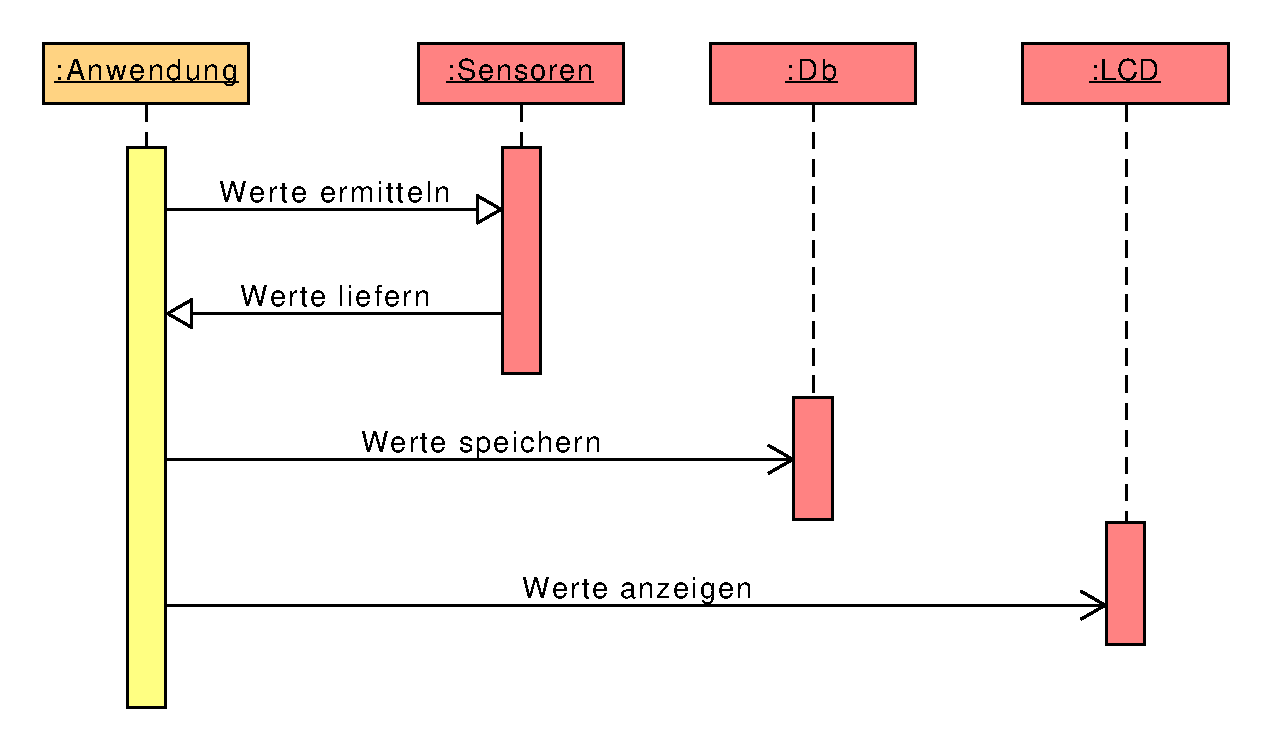
\includegraphics[width=\textwidth]{sequence-diagram}
    \caption{Sequenz Diagramm}
    \label{fig:sequence-diagram}
\end{figure}

\subsection{Struktur}
Die Anwendung befindet sich im laufenden Zustand, sobald das Gerät gestartet wird. Sie
wird bis zum Herunterfahren des Gerätes nicht mehr gestoppt. Es handelt sich also um einen
Dämon, welcher über geeignete Massnahmen dazu bewegt werden muss, die Werte auszulesen,
diese zu speichern und auf dem Display anzuzeigen. Zudem kann der Anwender die Anzeige auf
dem Display wechseln, resp. er kann den anzuzeigenden Wert wählen oder die IP Adresse
anzeigen lassen. Daher muss zusätzlich eine Möglichkeit bestehen, den Dämon zu
veranlassen, die Anzeige zu wechseln.

Das Auslesen und Abspeichern der Werte läuft vollkommen automatisch im Hintergrund ab,
diesen Vorgang kann der Benutzer nicht beeinflussen. Daher kann dies in einem eigenen
Thread abgearbeitet werden, welcher während der gesamten Laufzeit des Dämons aktiv ist.
Für den Wechsel der Anzeige muss der Dämon resp. die zugehörige Einheit auf Tastendruck
reagieren.

Zusammenfassend ergibt sich die Klassenstruktur wie sie in Abbildung
\ref{fig:class-diagram} dargestellt ist.

\begin{figure}[ht]
    \centering
    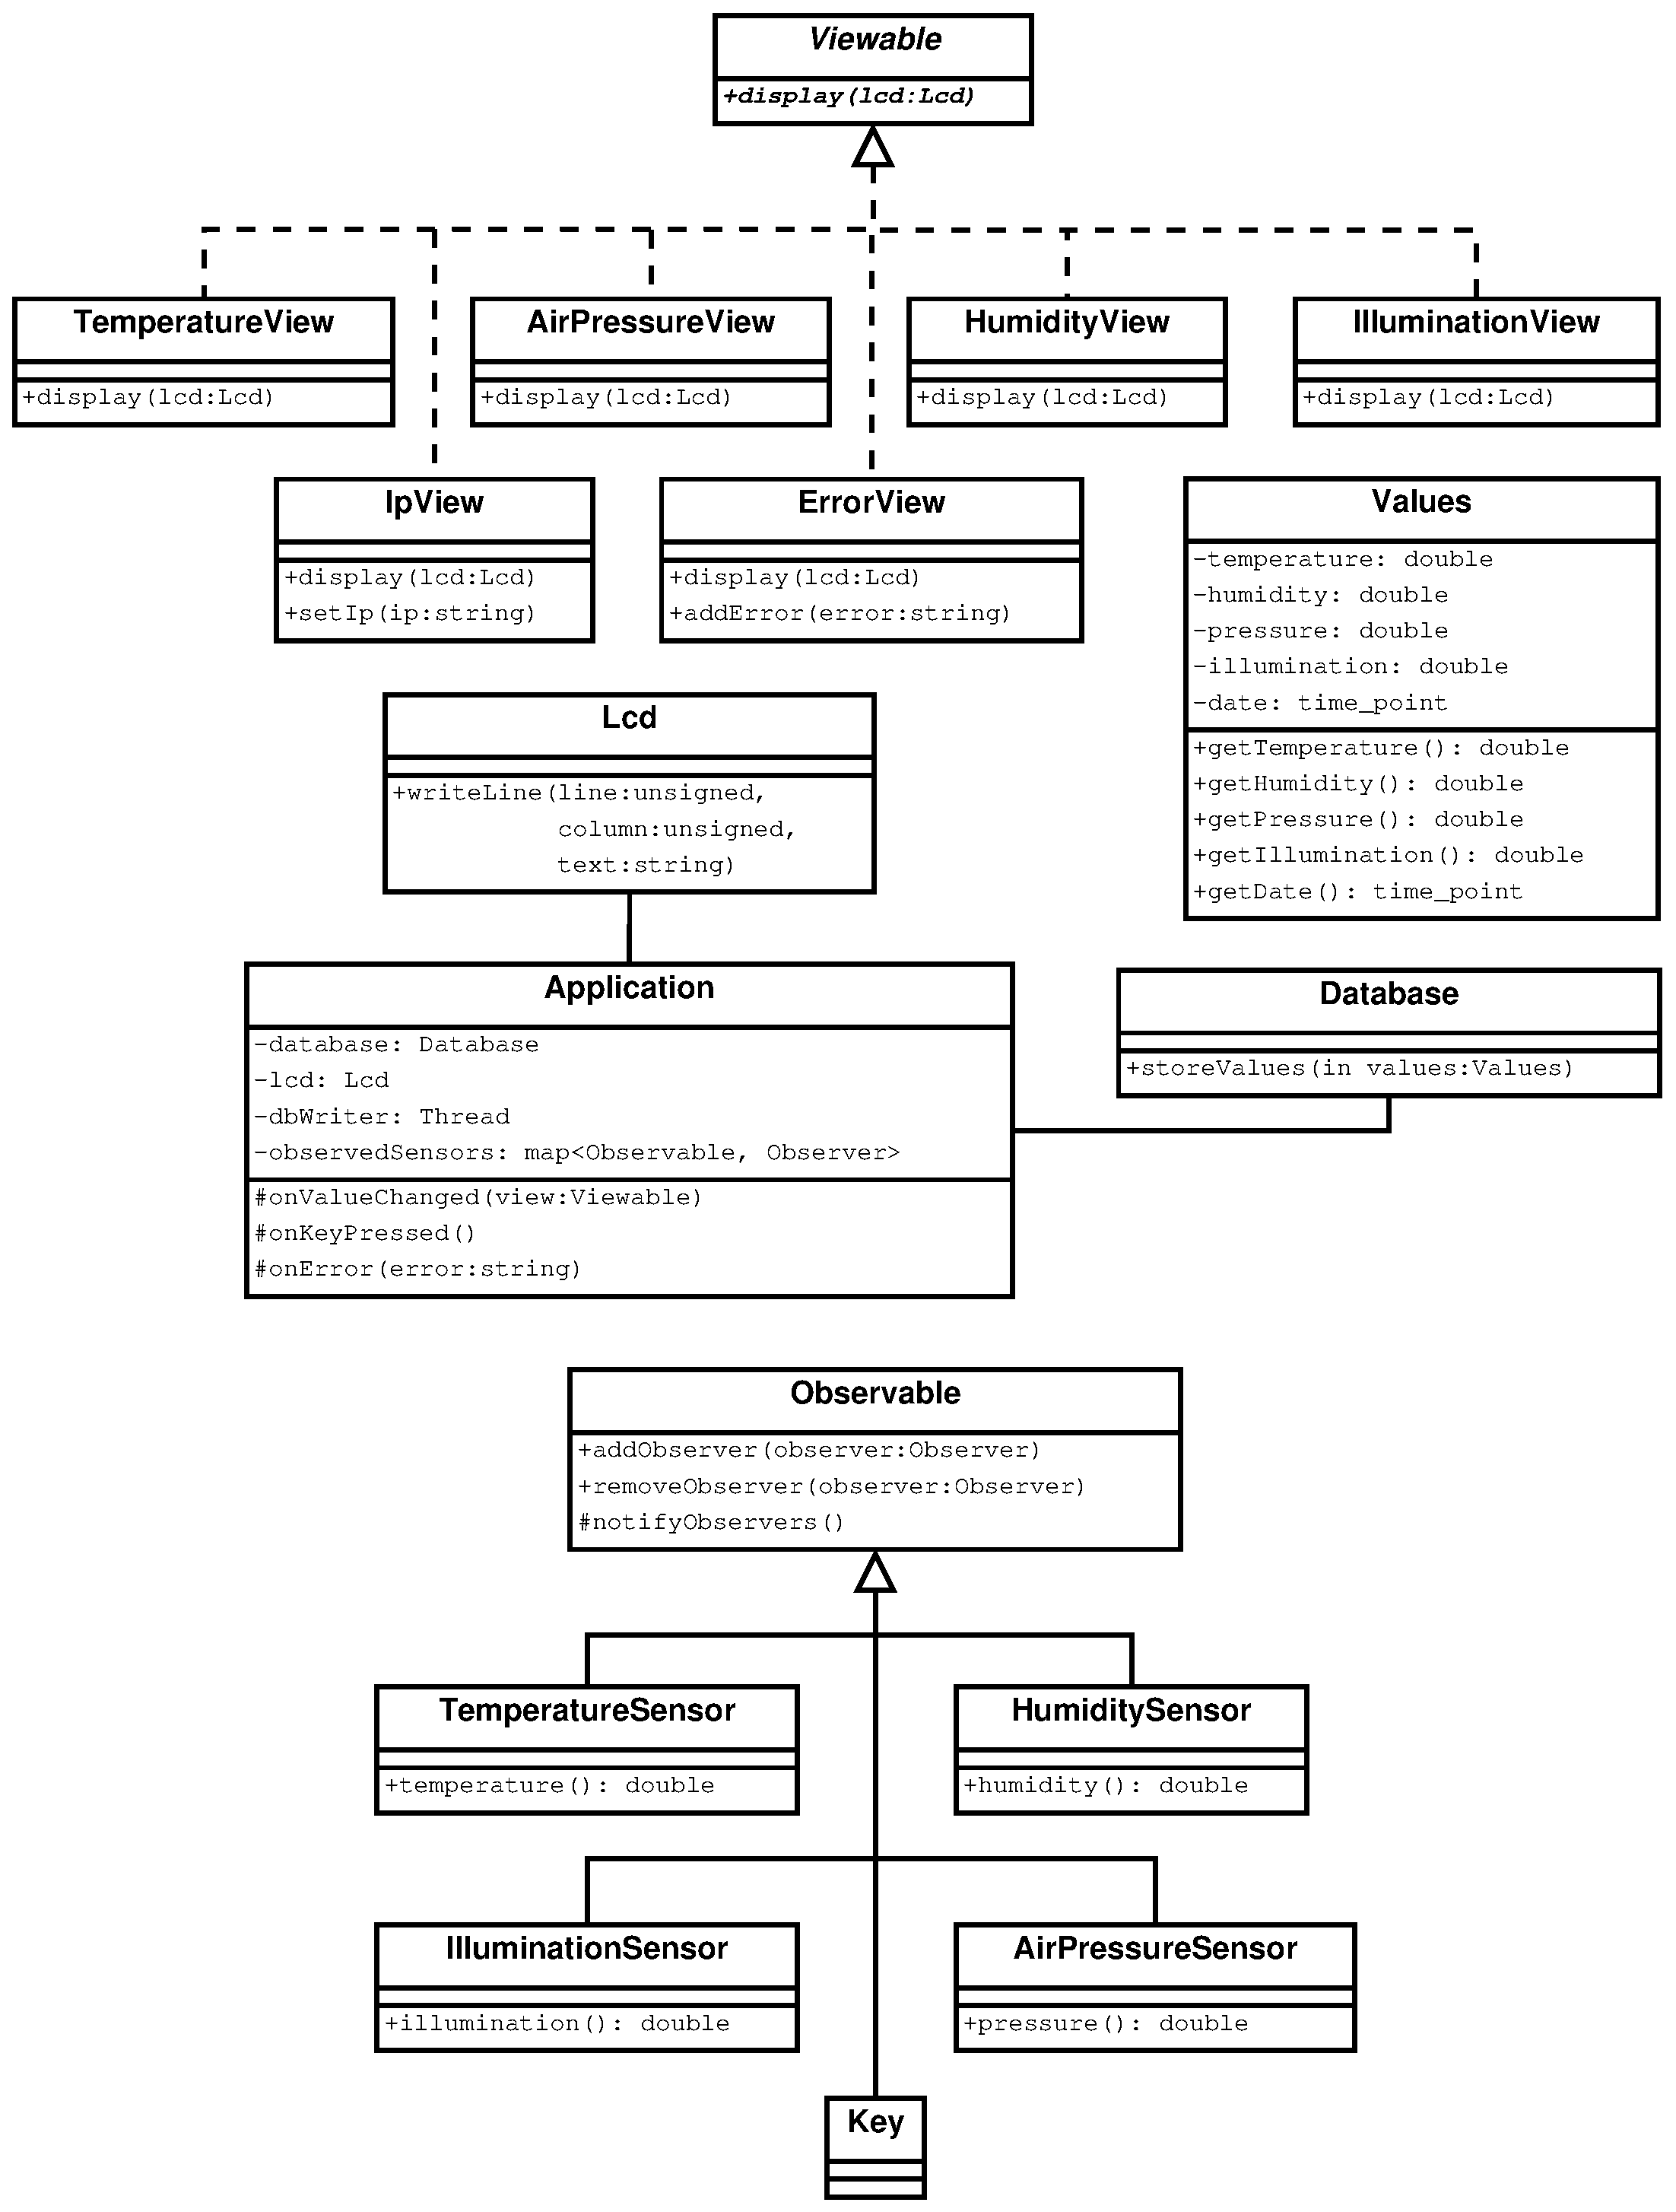
\includegraphics[width=\textwidth]{class-diagram.eps}
    \caption{Klassen Diagramm}
    \label{fig:class-diagram}
\end{figure}

% \FloatBarrier
% \appendix

% \listoftables
\listoffigures
% \lstlistoflistings
% \printglossary[title = Glossar, toctitle = Glossar]

\bibliographystyle{apacite}
\bibliography{02-software-on-pi}

% \renewcommand{\refname}{\section{Bibliographie}}
% \begin{thebibliography}{}
    % \bibitem[<+text+>]{<+name+>} <+author+>: <+book+>, <+publisher+>, <+year+>
% \end{thebibliography}<++>

\end{document}
